\documentclass[12pt]{article} % use larger type; default would be 10pt
\usepackage[utf8]{inputenc} % set input encoding (not needed with XeLaTeX)

%%% PAGE DIMENSIONS
\usepackage{geometry} % to change the page dimensions
\geometry{a4paper} % or letterpaper (US) or a5paper or....
\geometry{margin=2cm} % or letterpaper (US) or a5paper or....

\usepackage{graphicx} % support the \includegraphics command and options
\usepackage[parfill]{parskip} % Activate to begin paragraphs with an empty line rather than an indent
\usepackage{times} % for Times Roman default font

%%% PACKAGES
\usepackage{booktabs} % for much better looking tables
\usepackage{array} % for better arrays (eg matrices) in maths
\usepackage{paralist} % very flexible & customisable lists (eg. enumerate/itemize, etc.)
\usepackage{verbatim} % adds environment for commenting out blocks of text & for better verbatim
\usepackage{subfig} % make it possible to include more than one captioned figure/table in a single float

%%% HEADERS & FOOTERS
\usepackage{fancyhdr} % This should be set AFTER setting up the page geometry
\pagestyle{fancy} % options: empty , plain , fancy
\renewcommand{\headrulewidth}{0pt} % customise the layout...
\lhead{}\chead{}\rhead{}
\lfoot{}\cfoot{\thepage}\rfoot{}

\makeatletter
\renewcommand{\maketitle}{%
  {\bfseries{\scshape{\Large{\@title\par}}}}
}
\makeatother

\hyphenation{Kiwi-bank} % otherwise it may get hyphenated as Ki-wibank

%%% END Article customizations

%%% The "real" document content comes below...

\title{Alfred River Rock: May 2017}

\begin{document}
  \maketitle

Along the Alfred River, on the way to Lake Daniell, one finds the typical grey river rock (greywacke?), but occasionally there are tan-colour stones of a curious texture.  I asked John Begg about these and got the following reply:

``The picture you sent is very interesting. It looks to me like a tufa. Tufa is a  porous rock composed largely of calcium carbonate formed by precipitation from saturated water around mineral springs. The rod-like things in it are `fossilised' twigs or moss. My bet is it will be young (Holocene,  less than 6000 years old), and the saturated spring water may even come from a fault zone that brings deep, mineral-saturated water to the surface. When it comes in contact with the low pressure and temperature conditions, the CaCO3 precipitates out, `fossilising' any surficial organic materials it is in contact with.''

\begin{figure}[hb]
%\centering
\begin{center}
   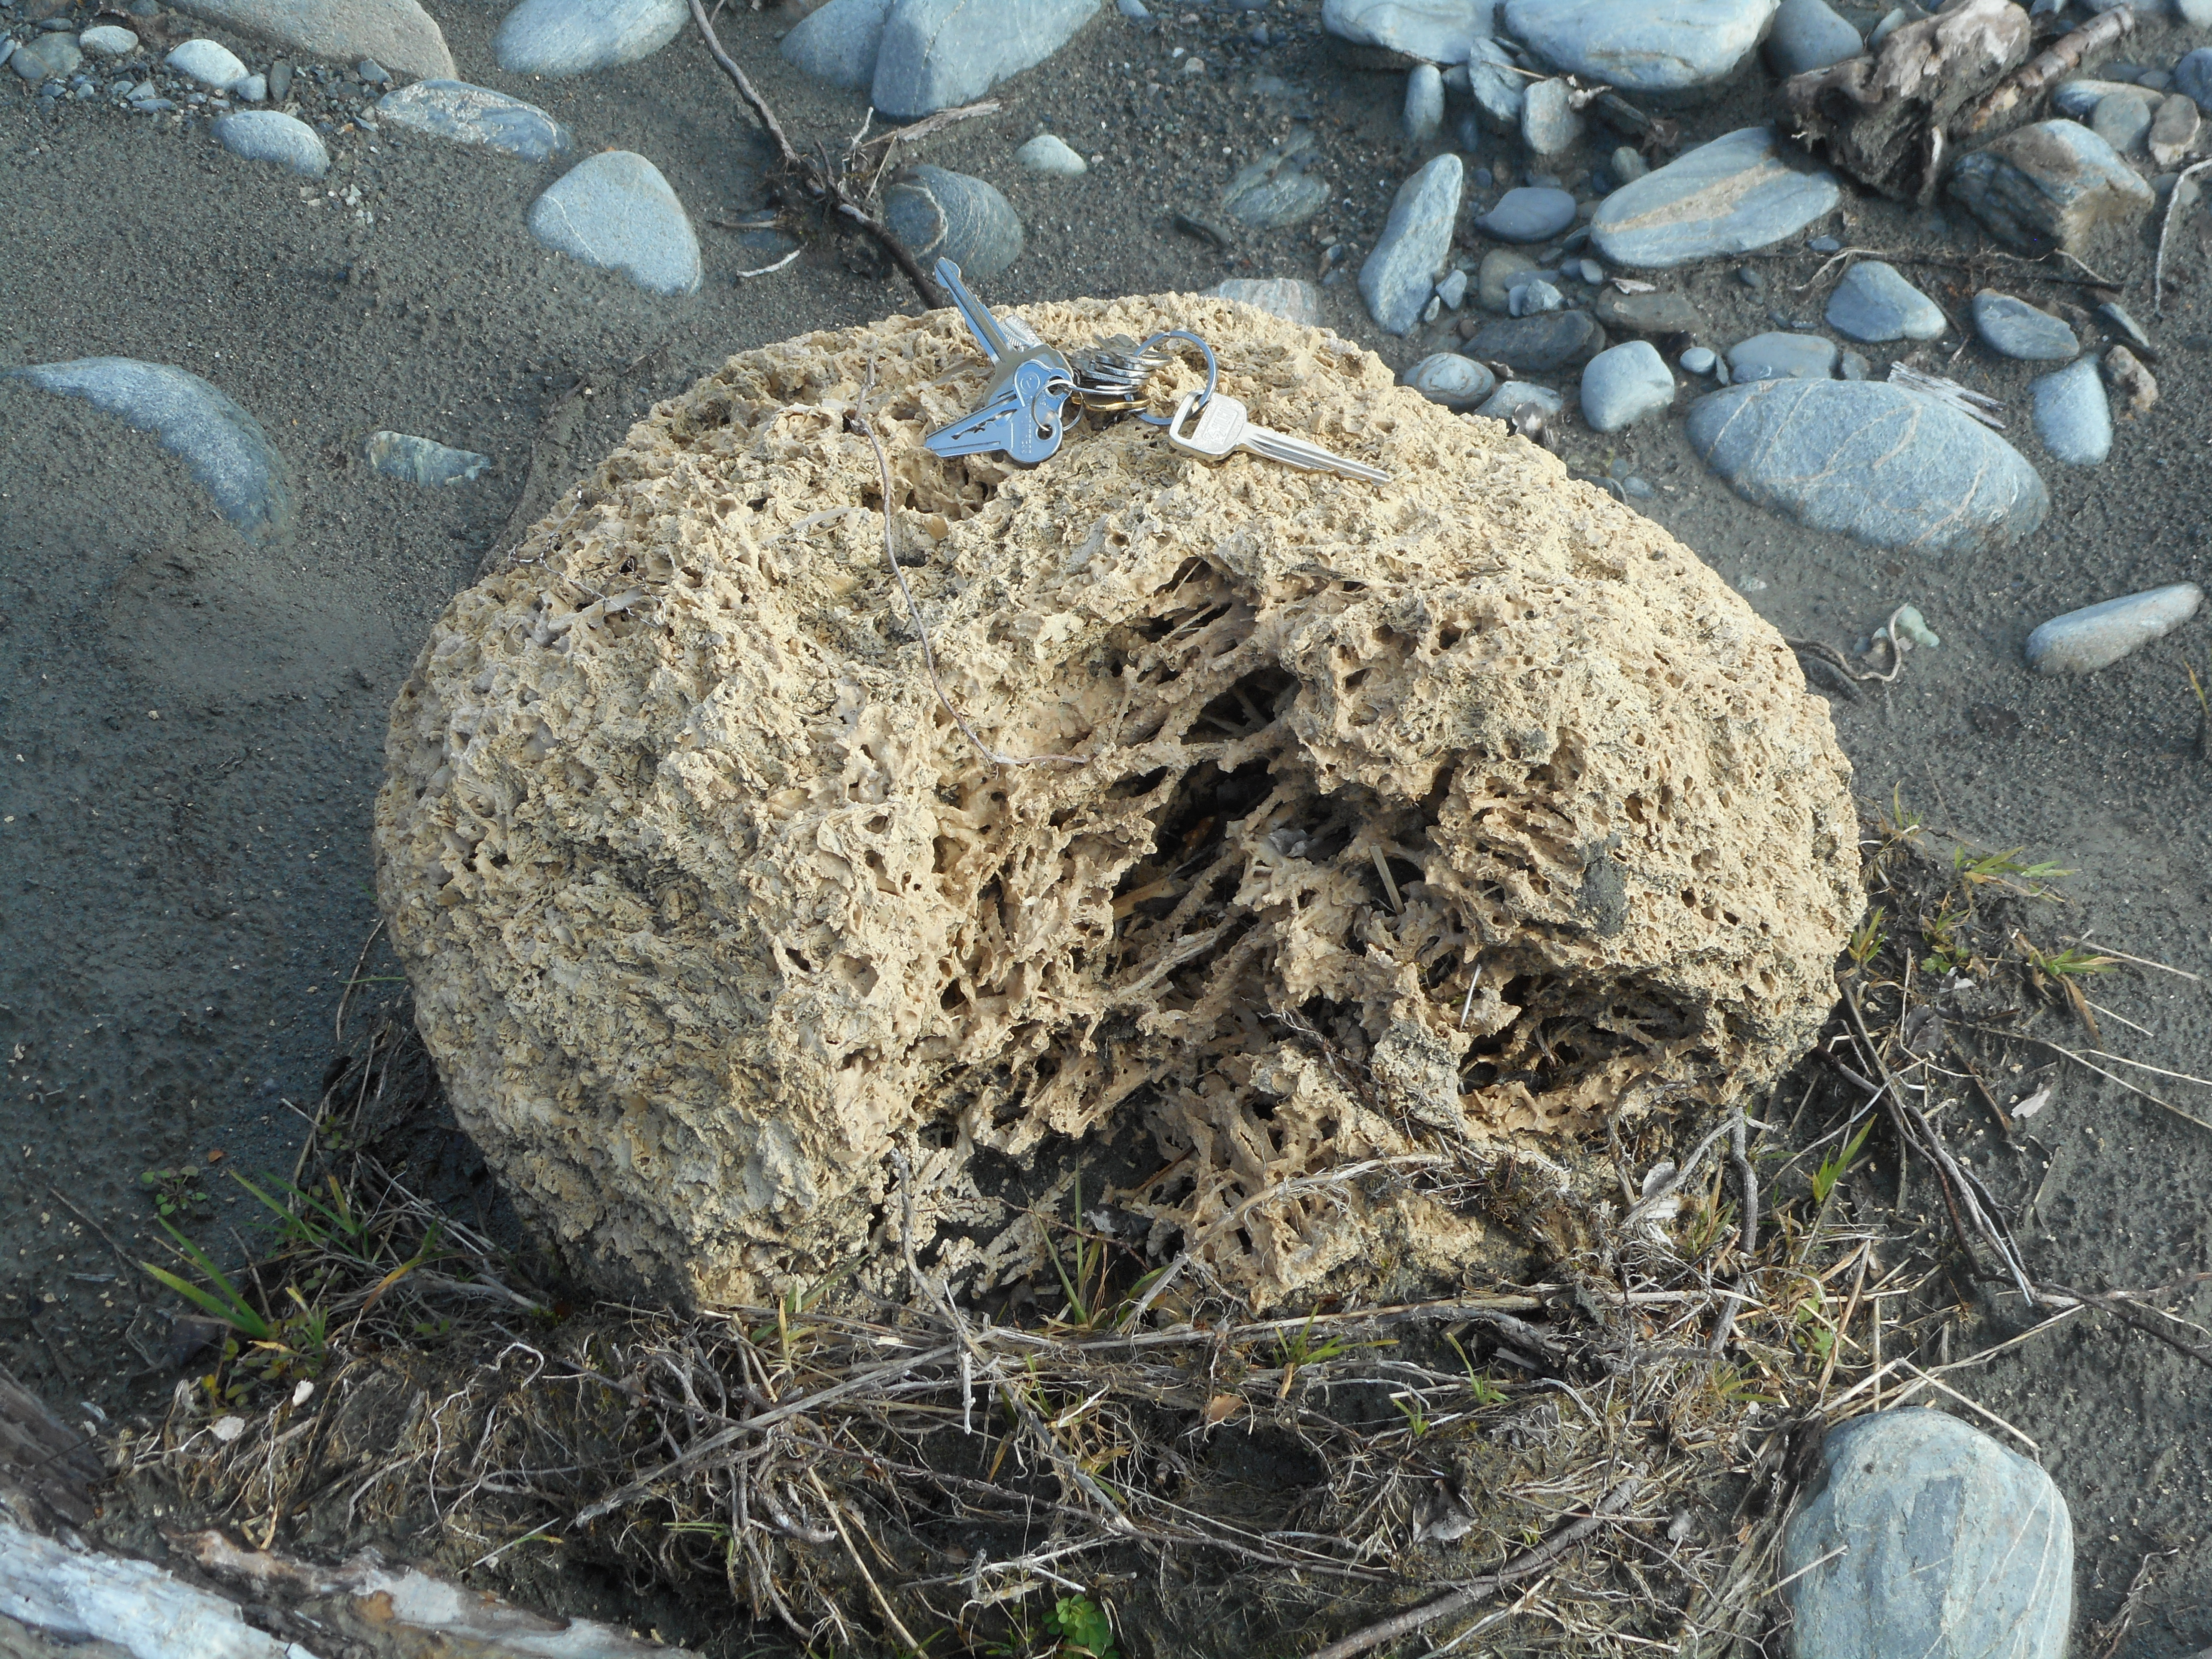
\includegraphics[width=12cm]{AlfredRiverRockPhoto}
\end{center}
\end{figure}

\end{document}
